\documentclass[10pt]{exam}
\usepackage[icp]{template-for-exam}
\usepackage{pgfplots}
\pgfplotsset{
    compat=1.18,
    reg/.append style={
        xmin =-4.5,
        xmax =4.5,
        ymin =-4.5,
        ymax = 4.5,
        axis lines = center,
        xtick = {-4,...,4},
        ytick = {-4,...,4},
        height = 6cm,
        width = 6cm,
        grid = major,
        grid style = {thick, dotted},
        tick label style = {font=\small}
      },
    myplot/.append style={
      smooth,domain=-4:4,samples=50,thick
    },
  }

\title{Reading Guide - Interference}
\author{Rohrbach}
\date{\today}

\begin{document}
\maketitle

\begin{questions}


\uplevel{Read about interference on pp. 510-511.}

\question
  What is interference?
  \vs

\question
  What are the two types of interference and what are their definitions?
  \vs

\question
  Look at figure 12 on page 511.   Read the entire caption.  How is he amplitude of wave 3 related to the amplitudes of waves 1 and 2?
  \vs

\question
  With your instructor, draw constructive interference and destructive interference
  \vs

\end{questions}

\pagebreak

\noindent
Draw the resulting wave in each of the following cases:


\begin{center}
  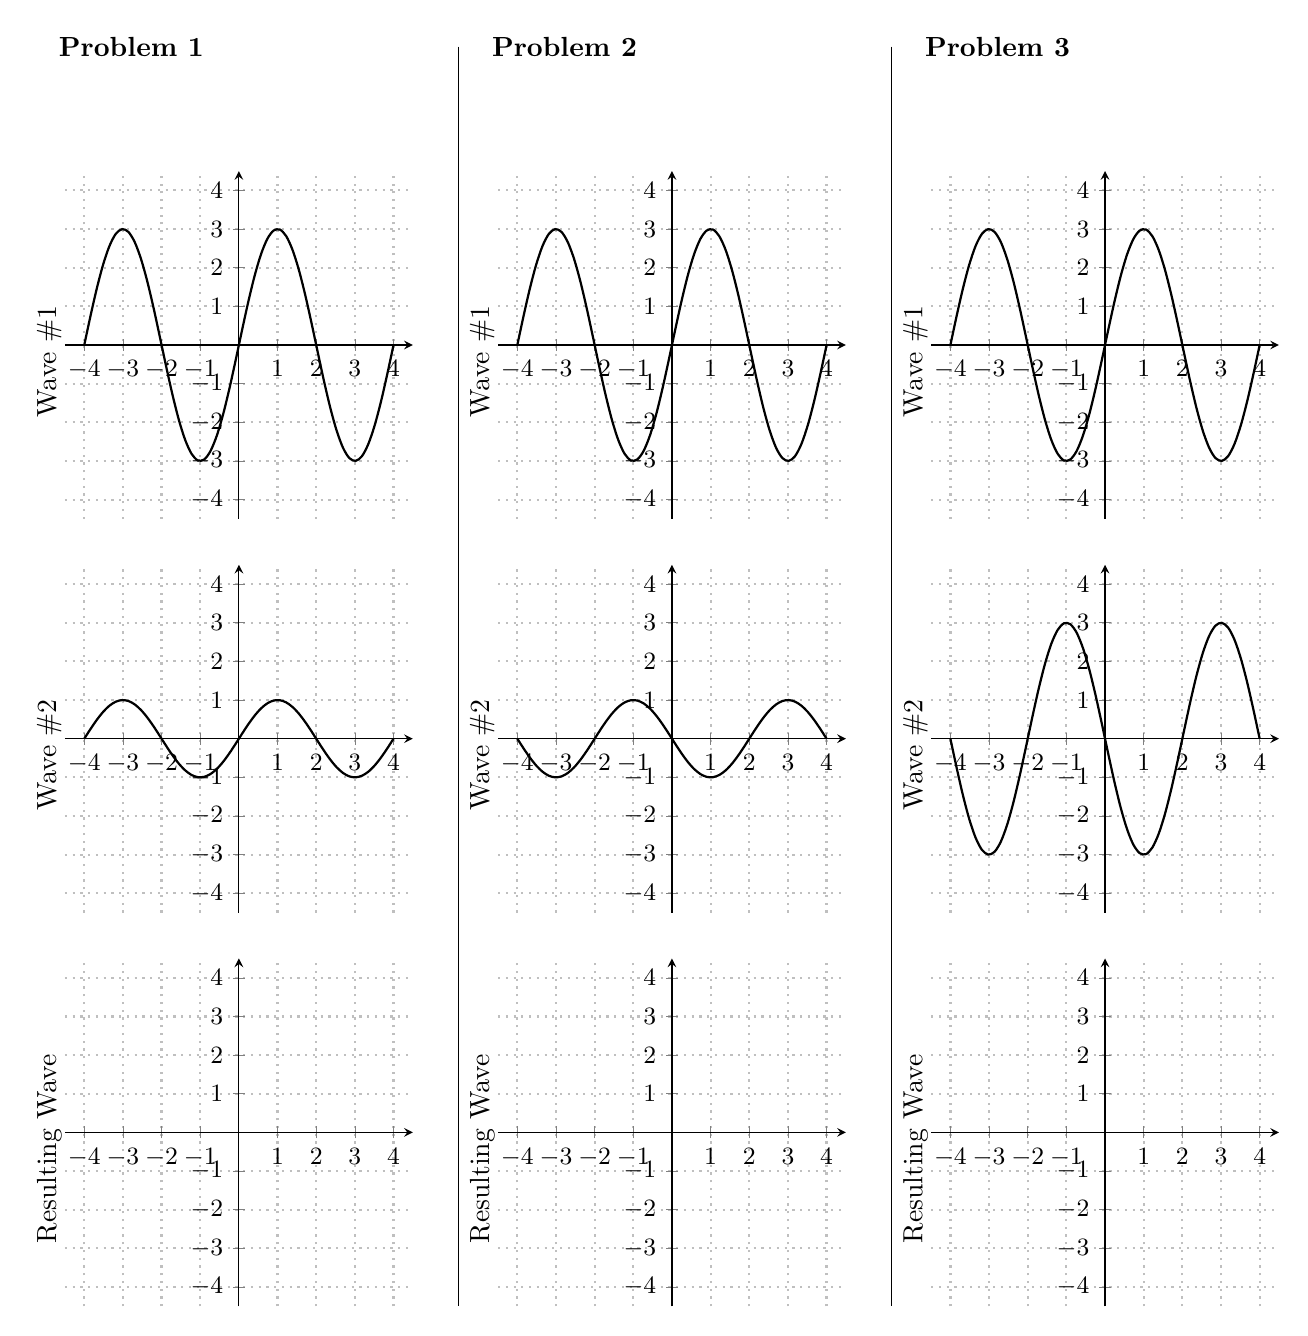
\begin{tikzpicture}
    \draw (5,6)  -- ++(0,-16);
    \draw (10.5,6)  -- ++(0,-16);
  
    \begin{scope}
      \node[anchor=west] at (-.2,6) {\bf Problem 1};
      \begin{scope}
          \node[rotate=90] at (-.2,2) {Wave \#1};
          \begin{axis}[reg]
            \addplot[myplot] {3*sin(deg(2*pi*x/4))};
          \end{axis}
      \end{scope}
      
      \begin{scope}[shift={(0,-5)}]
        \node[rotate=90] at (-.2,2) {Wave \#2};
        \begin{axis}[reg]
          \addplot[myplot] {1*sin(deg(2*pi*x/4))};
        \end{axis}
      \end{scope}
  
      \begin{scope}[shift={(0,-10)}]
        \node[rotate=90] at (-.2,2) {Resulting Wave};
        \begin{axis}[reg]
        \end{axis}
      \end{scope}
  
    \end{scope}
      
    \begin{scope}[shift={(5.5,0)}]
  
      \node[anchor=west] at (-.2,6) {\bf Problem 2};
      \begin{scope}
        \node[rotate=90] at (-.2,2) {Wave \#1};
          \begin{axis}[reg]
            \addplot[myplot] {3*sin(deg(2*pi*x/4))};
          \end{axis}
      \end{scope}
      
      \begin{scope}[shift={(0,-5)}]
        \node[rotate=90] at (-.2,2) {Wave \#2};
        \begin{axis}[reg]
          \addplot[myplot] {-1*sin(deg(2*pi*x/4))};
        \end{axis}
      \end{scope}
  
      \begin{scope}[shift={(0,-10)}]
        \node[rotate=90] at (-.2,2) {Resulting Wave};
        \begin{axis}[reg]
        \end{axis}
      \end{scope}
  
    \end{scope}
  
    \begin{scope}[shift={(11,0)}]
  
      \node[anchor=west] at (-.2,6) {\bf Problem 3};
      \begin{scope}
        \node[rotate=90] at (-.2,2) {Wave \#1};
          \begin{axis}[reg]
            \addplot[myplot] {3*sin(deg(2*pi*x/4))};
          \end{axis}
      \end{scope}
      
      \begin{scope}[shift={(0,-5)}]
        \node[rotate=90] at (-.2,2) {Wave \#2};
        \begin{axis}[reg]
          \addplot[myplot] {-3*sin(deg(2*pi*x/4))};
        \end{axis}
      \end{scope}
  
      \begin{scope}[shift={(0,-10)}]
        \node[rotate=90] at (-.2,2) {Resulting Wave};
        \begin{axis}[reg]
        \end{axis}
      \end{scope}
  
    \end{scope}
  
  \end{tikzpicture}
\end{center}


\end{document}